
\paragraph{Monkeys exhibit biases} %hallmarks of color category behavior

The animals examined show a hallmark of color categorization behavior: memory biases towards a set of particular points in a perceptually uniform colorspace.
In \autoref{fig:AvResults} it can be seen that the biases deviate substantially and systematically from zero, with the attractor points being found where the bias line crosses the zero line from positive to negative (going counter-clockwise). These points are highlighted with colored lines, with the filled areas around these lines showing the confidence intervals on these crossing points. Repeller points found where the line crosses the zero line from negative to positive.

\begin{figure}
    \centering
    \begin{subfigure}[b]{\textwidth}
         \centering
         \caption{}
         \includesvg[pretex=\tiny, width=\textwidth]{../Figures/working/2_AvResults/combined_categorybias1_230214.svg}
         \label{fig:CombinedLinear}
    \end{subfigure}
    \hfill
    \begin{subfigure}[b]{\textwidth}
         \centering
         \caption{}
         \includesvg[pretex=\tiny, width=\textwidth]{../Figures/working/2_AvResults/combined_categorybias2_230214.svg}
         \label{fig:CombinedPolar}
    \end{subfigure}
    \caption{\textbf{Bias as a function of hue, for data collapsed over 4 animals.} 
    }
    \label{fig:AvResults}
\end{figure}

\paragraph{Shared color categories across monkeys}

We see that all tested monkeys share two common attractor points (\autoref{fig:BiasCurvesIndividual}), which we interpret as evidence of two shared color categories: a warm/orange-ish category (between 0$^\circ$ and 45$^\circ$), and a cool/blue-ish category (between 180$^\circ$ and 225$^\circ$). 

% Results table?

%\begin{figure}
%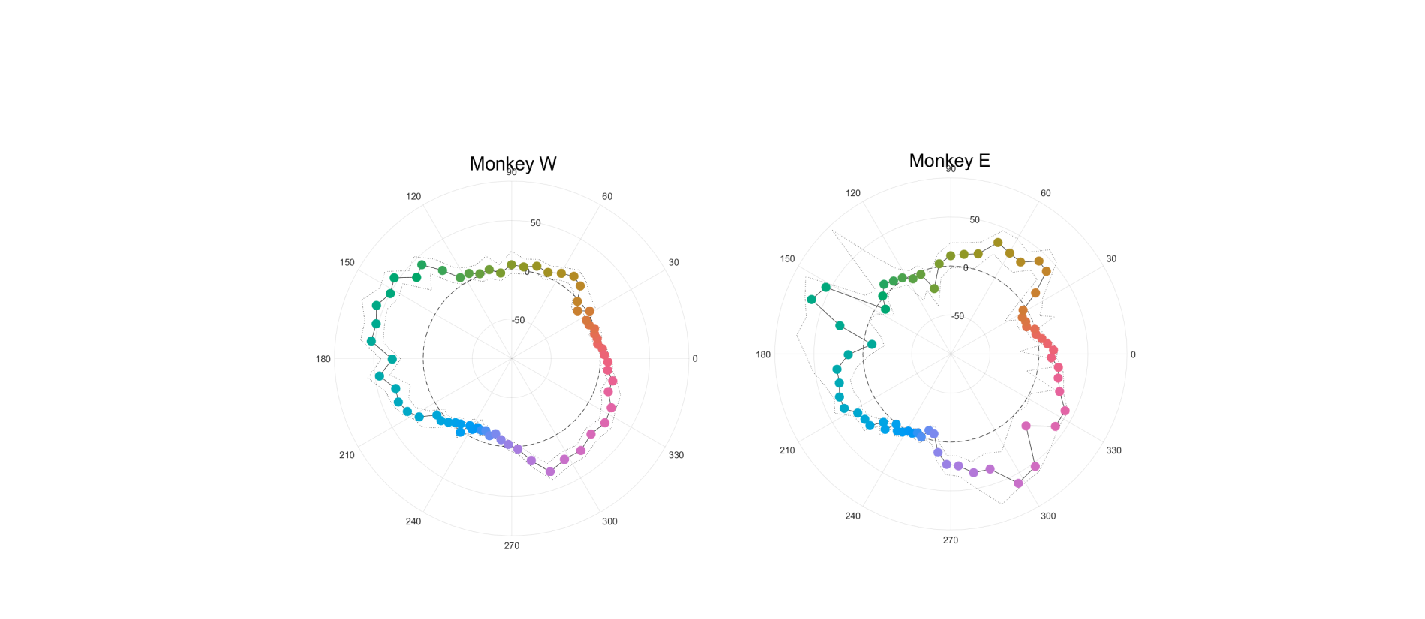
\includegraphics[width=\textwidth]{../../Figures/Old/panichellobias.pdf}
%\caption{Bias as a function of hue, for Panichello monkeys} 
%\end{figure}

\paragraph{Biases Compared to Humans}

Comparison to our human data, Mech Turk and also rig (maybe?)

Comparison to \cite{bae_why_2015}

Comparison to \cite{panichello_error-correcting_2019}

\paragraph{Cognitive Bias vs. Non-uniformity in Perceptual Space}

\begin{figure}
    \centering
    \begin{subfigure}[b]{0.49\textwidth}
         \centering
         \caption{}
        \includesvg[pretex=\tiny, width=\textwidth]{../Figures/working/3_TCCDemo/simdata_skewedGaus_categorybias2_230707.svg}
         \label{fig:JustBias}
    \end{subfigure}
    \hfill
    \begin{subfigure}[b]{0.49\textwidth}
         \centering
         \caption{}
         \includesvg[pretex=\tiny, width=\textwidth]{../Figures/working/3_TCCDemo/simdata_ssnu_categorybias2_230707.svg}
         \label{fig:JustColSpace}
    \end{subfigure}

    \begin{subfigure}[b]{0.49\textwidth}
         \centering
         \caption{}
         \includesvg[pretex=\tiny, width=\textwidth]{../Figures/working/3_TCCDemo/skewedGaus_sm_230707.svg}
         \label{fig:JustBias_subset}
    \end{subfigure}
    \hfill
    \begin{subfigure}[b]{0.49\textwidth}
         \centering
         \caption{}
         \includesvg[pretex=\tiny, width=\textwidth]{../Figures/working/3_TCCDemo/sm_ssnu_230707.svg}git pull
         \label{fig:JustColSpace_subset}
    \end{subfigure}
        \caption{\textbf{Distinguishing between different sources of bias using TCC models: cognitive bias vs. non-uniformity of stimulus space.} Similarity matrices representing different theoretically driven mechanisms can result in the same average bias value. A mixture model cannot distinguish between these different sources, whereas a TCC model readily can. \ref{fig:JustBias}: an example of how cognitive bias might appear - each row of the matrix is shifted leftwards or rightwards. \ref{fig:JustColSpace}: an example of how non-uniformity in stimulus space might appear - the similarity between each cue and its neighbors is increased or decreased, resulting in an expansion of the higher similarity region of the matrix symmetrically around the negative diagonal for colors which are more similar to their neighbors than average, and a contraction for colors that are less similar to their neighbors than average. \ref{fig:JustBias_subset}: The values representing the similarity function for cue 20 (the row highlighted in red in \ref{fig:JustBias}), with the circular median shown as a vertical dashed line. \ref{fig:JustColSpace_subset}: As in \ref{fig:JustBias_subset} but for \ref{fig:JustColSpace}. Note how the circular median of \emph{both} functions is 25.}
        \label{fig:TCCDemo}
        % !! update this to mirror the VSS 2023 poster with the mixture model examples?
\end{figure}

\begin{figure}
    \centering
    \begin{subfigure}[b]{0.49\textwidth}
         \centering
         \caption{}
         \includesvg[pretex=\tiny, width=\textwidth]{../Figures/working/4_TCCOutput/combined_TCC-FreeSimilarityMatrix_230509.svg}
         \label{fig:SimilarityMatrixCombined}
    \end{subfigure}
    \hfill
    \begin{subfigure}[b]{0.49\textwidth}
         \centering
         \caption{}
         \includesvg[pretex=\tiny, width=\textwidth]{../Figures/working/4_TCCOutput/combined_TCC-0att_fullremap-similaityMatrix_230510.svg}
         \label{fig:SimilarityMatrixCombinedRemapOnly}
    \end{subfigure}
    \caption{\textbf{Free Similarity model fit for combined data from all animals.}
    Similarity between stimulus $s_i$ and stimulus $s_j$, where one is the cue and one is the choice. This is a ``free'' similarity matrix - in that no particular relationship is pre-supposed between any of the stimuli (such as, for example: closer stimuli will be more similar). This figure can be compared to Figure 1D in \cite{schurgin_psychophysical_2020}, except there the rows are circularly shifted so that the the x-axis becomes the relative distance, rather than the absolute value of the stimulus. % should we just plot it the same way at this stage? It doesn't really make a difference here...
    % supplementary figure with alternative plotting method?
    %confidence intervals?!?!?! !!!!!!!!!!!!!!
    } 
    \label{fig:TCCOutput}
\end{figure}

\paragraph{A behaviorally-derived colorspace}

Extracted colorspace shown in \autoref{fig:MACBEHcolorspace}.

\begin{figure}
    \centering
    \begin{subfigure}[b]{0.3\textwidth}
         \centering
         \caption{Stimuli in CIELUV \newline\newline}
         \includesvg[pretex=\tiny, width=\textwidth]{../Figures/working/5_ColSpace/colorspace_230511.svg}
         \label{fig:CIELUV}
    \end{subfigure}
    \hfill
    \begin{subfigure}[b]{0.3\textwidth}
         \centering
         \caption{Stimuli in behaviorally-derived space \newline}
         \includesvg[pretex=\tiny, width=\textwidth]{../Figures/working/5_ColSpace/behaviorally-derived-colorspace_230630.svg}
         \label{fig:MACBEHspace}
    \end{subfigure}
    \hfill
    \begin{subfigure}[b]{0.3\textwidth}
         \centering
         \caption{Stimuli sampled in behaviorally-derived space, projected back into CIELUV}
         \includegraphics[width=\textwidth]{example-image-a}
         \label{fig:UniformStimsInCIELUV}
    \end{subfigure}
           \caption{\textbf{A behaviorally-derived colorspace.} Ipsum!}
        \label{fig:MACBEHcolorspace}
    
\end{figure}

\paragraph{Individual differences between monkeys}

In one animal \autoref{fig:BiasCurvesCastor} we see evidence of additional categories: strong evidence for a greenish category and weak evidence for a purple category (the ``strength" of a category can be gleaned from looking at the local gradient at the zero-crossing point)

\begin{figure}
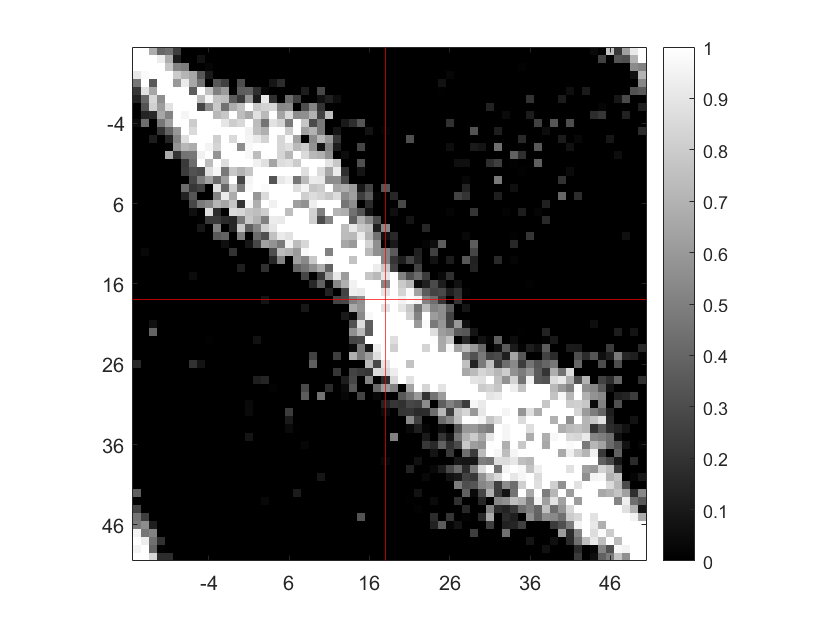
\includegraphics[width=\linewidth]{../Figures/working/6_IndiDataCogBias/Castor_18.png}
\caption{\textbf{} 
}
\label{fig:IndiDataCogBias}
\end{figure}